\section{Invasive Species Trade-Off Model Discussion}

\subsection{Model Generalization}

When applying our model to a larger sample of foreign plants to classify them as invasive or not invasive, it would be immensely beneficial to create an auto-classification system. Such a classification system would consist of a "line of division" in a plot where each axis would represent the ecological or economic scores. Since we do not have enough data points to create such a classification system, we design a \textit{DSD} framework (Data-Score-Divide) below where an environmental scientist may use our trade-off model.

In our proposed \textit{DSD} framework, environmental scientists would perform the following steps as described in Figure~\ref{fig:dsdprocess}. First, a scientist must collect regional native population data, economic costs and revenues from similar firms, and determine dollar-value human risk costs in local populations. Next, data is to be evaluated via our proposed ecological and economic scores. Finally, scores for each foreign species should be plotted on an economic versus ecological score plot, where a line of division must be drawn by an evaluator to specify the split between invasive and simply foreign species. This division process is inspired by Support Vector Machines, which are commonly used in machine learning classification tasks \cite{ieeeSupportVector}.

We did not conduct a sensitivity analysis on our trade-off model because, in a sense, the environmental scientists who \textit{divide} the scores are the primary influences of the final decision.

\begin{figure}[h!]
\centering
    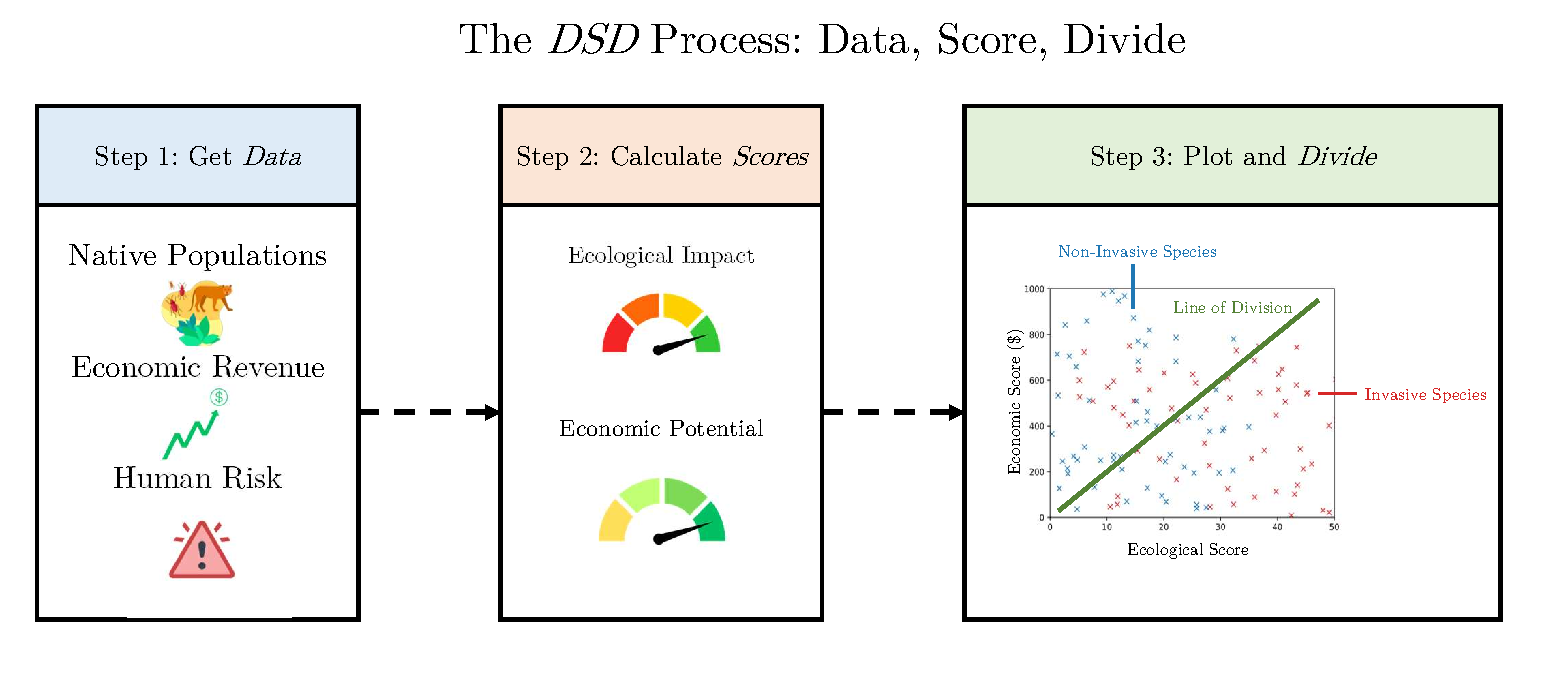
\includegraphics[scale=0.6]{figures/dsdprocess.pdf}
    \captionsetup{width=0.9\textwidth}
    \caption{\textbf{The \textit{Data-Score-Divide} (DSD) framework for evaluating foreign species.}}
    \label{fig:dsdprocess}
\end{figure}

\subsection{Strengths}
\begin{enumerate}
    \item Our model offers unique\textbf{ insights into the trade-offs} of foreign species, in particular, invasive species.
    \begin{quote}
        Unlike impact models that only examine the ecological benefits and downfalls of a foreign species, our model examines both ecological and economic trade-offs.
    \end{quote}
    \item Our model is adaptable to virtually \textbf{any region and foreign plant} combination.
    \begin{quote}
        This means that our model can be applied to different scenarios and contexts, such as invasive species management, biodiversity conservation, and ecological restoration. Our model can adapt based on different regional native plants and economic conditions. We also provide a general-use framework that can be quickly applied to many species at a time.
    \end{quote}
\end{enumerate}
\subsection{Limitations}
\begin{enumerate}
\item Intra-population dynamics between foreign and native species that are unknown \textbf{can be difficult to predict}.
    \begin{quote}
     In the previous three contexts of analyzing the trade-offs between dandelion, garlic mustard, and English ivy plants, the most distinct aspect of these species is that they are widely classified as invasive or a "weed." This means that for unknown foreign species relationships, scientists must input some observational data into the model.
    \end{quote}
\item New economic benefits and pitfalls \textbf{may not follow historical trends}.
\begin{quote}
    In our analysis of dandelion and English ivy plants, several businesses centered around dandelion and English ivy harvesting already exist. This allows us to build upon previous work to calculate new economic profits and yield. However, when we take a look at the case of garlic mustard plants, few garlic mustard firms exist, which hinders our ability to predict economic outcomes.
\end{quote}
    
\end{enumerate}

